\documentclass[11pt]{amsart}
\usepackage{geometry}                % See geometry.pdf to learn the layout options. There are lots.
\geometry{letterpaper}                   % ... or a4paper or a5paper or ... 
%\geometry{landscape}                % Activate for for rotated page geometry
%\usepackage[parfill]{parskip}    % Activate to begin paragraphs with an empty line rather than an indent
\usepackage{graphicx}
\usepackage{amssymb}
\usepackage{epstopdf}
\usepackage{graphicx}
\usepackage{siunitx}
\usepackage[backend=biber]{biblatex}
\bibliography{clock-gears.bib}

\DeclareGraphicsRule{.tif}{png}{.png}{`convert #1 `dirname #1`/`basename #1 .tif`.png}

\title{Clock Gears}
\author{Steven R. Loomis}
\date{}                                           % Activate to display a given date or no date

\begin{document}
\maketitle

\begin{figure}[h!]
  \caption{A 60 tooth gear.}
  \centering
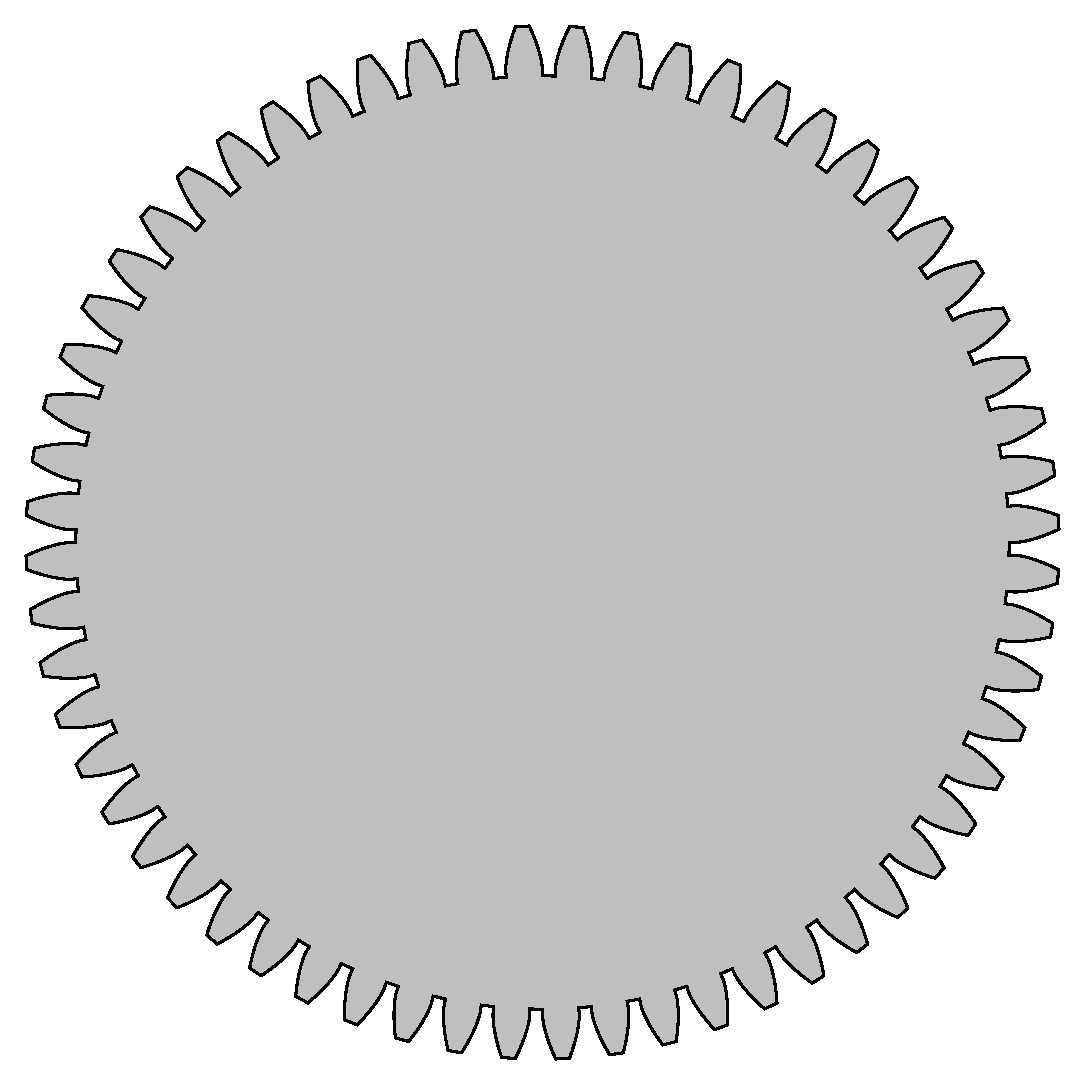
\includegraphics[width=1in]{gear.pdf}
\end{figure}

\section{Intro}

I have a son who loves gears and clocks.  I work on date and time stuff. Someday, I hope we can build a clock together. In the mean time,
I've done some calculations on what the clock gears should look like. For a great reference on date and time, see \citation{calendrical}.

\section{Calculation}

\subsection{Basic Day Math}

There are 60 seconds in a minute.

There are 60 minutes in an hour, thus, 3,600 seconds in an hour.

There are 12 hours in half a day, or 24 hours in a full day.
There are 43,200 seconds in half a day, or 86,400 seconds in a full day.
There are 720 minutes in half a day, or 1,440 minutes in a full day.

\subsection{Between hands}

The second hand turns around once per minute. As there are 60 seconds in a minute, the second hand turns \( \frac{ \ang{360} }{60} = \ang{6} \)  per second.

The minute hand turns around once per hour. As there are 60 minutes in an hour, the minute hand turns  \( \frac{ \ang{360} }{60} = \ang{6} \)  per minute or 
  \( \frac{ \ang{360} }{3600} = \ang{0.1} = \ang{0;6;0} \) per second. 

The hour hand turns around once per half-day. As there are 12 hours in a half-day, the minute hand turns
 \( \frac{ \ang{360} }{12} = \ang{30} \)  per hour. 
 
 \subsection{Gearing}
 
 The gearing between Second and Minute hand is 60:1 that is 60 minutes per hour.
 
 The gearing between Minute and Hour hand is \( (60*12):1 = 720:1 \) that is 720 minutes in 12 hours.

\section{References}
\printbibliography

Gear image generated with https://github.com/cochrane/Gearmaker

\section{License}
This work is licensed under the Creative Commons Attribution-ShareAlike 4.0 International License. To view a copy of this license, visit http://creativecommons.org/licenses/by-sa/4.0/ or send a letter to Creative Commons, PO Box 1866, Mountain View, CA 94042, USA.

\begin{figure}[h!]
  \caption{CC-BY-SA-4.0 logo}
  \centering

\includegraphics[width=1in]{by-sa-4.png}
\end{figure}

\end{document}  
